\section{Introduction}
Machine perception systems have witnessed significant progress in the past years.
% thanks to the emergence of convolutional neural networks.
% ~\cite{lecun1998gradient,he2016deep,ren2015faster}.
Yet, our ability to train models that generalize to novel concepts without abundant labeled data is still far from satisfactory  when compared to human visual systems. 
Even a toddler can easily recognize a new concept with very little instruction~\cite{landau1988importance,samuelson2005they,smith2002object}.

The ability to generalize from only a few examples (so called few-shot learning) has become a key area of interest in the machine learning community.
Many \cite{vinyals2016matching,snell2017prototypical,finn2017model,hariharan2017low,gidaris2018dynamic,wang2019tafe} have explored techniques to transfer knowledge from the data-abundant base classes to the data-scarce novel classes through \emph{meta-learning}. 
They use simulated few-shot tasks by sampling from base classes during training to learn to learn from the few examples in the novel classes.

However, much of this work has focused on basic image classification tasks. 
In contrast, few-shot object detection has received far less attention. 
Unlike image classification, object detection requires the model to not only recognize the object types but also localize the targets among millions of potential regions. This additional subtask substantially
raises the overall complexity. Several~\cite{kang2019few,yan2019meta,wang2019meta} have attempted to tackle the under-explored few-shot object detection task, where only a few labeled bounding boxes are available for novel classes. These methods attach meta learners to existing object detection networks, following the meta-learning methods for classification. But, current evaluation protocols suffer from statistical unreliability, and the accuracy of baseline methods, especially simple fine-tuning, on few-object detection are not consistent in the literature.

% \fisher{will move.} Meta-learning based approaches seem to be promising in both few-shot classification as well as detection. However, some~\cite{chen2019closer} 
% raise concerns about the reliability of the results given 
% that a consistent comparison analysis of different approaches is missing. 
% Some simple fine-tuning based approaches, which draw little attention in the
% community, turn out to be more favorable than many prior works that use meta-learning
% on few-shot image classification~\cite{chen2019closer,dhillon2019baseline}.
% As for the emerging few-shot object detection task, there is no consensus on the evaluation benchmarks nor a consistent comparison of different approaches due to the increased network complexity, various implementation details, and variances in evaluation protocols.


\begin{figure*}[ht]
    \centering
    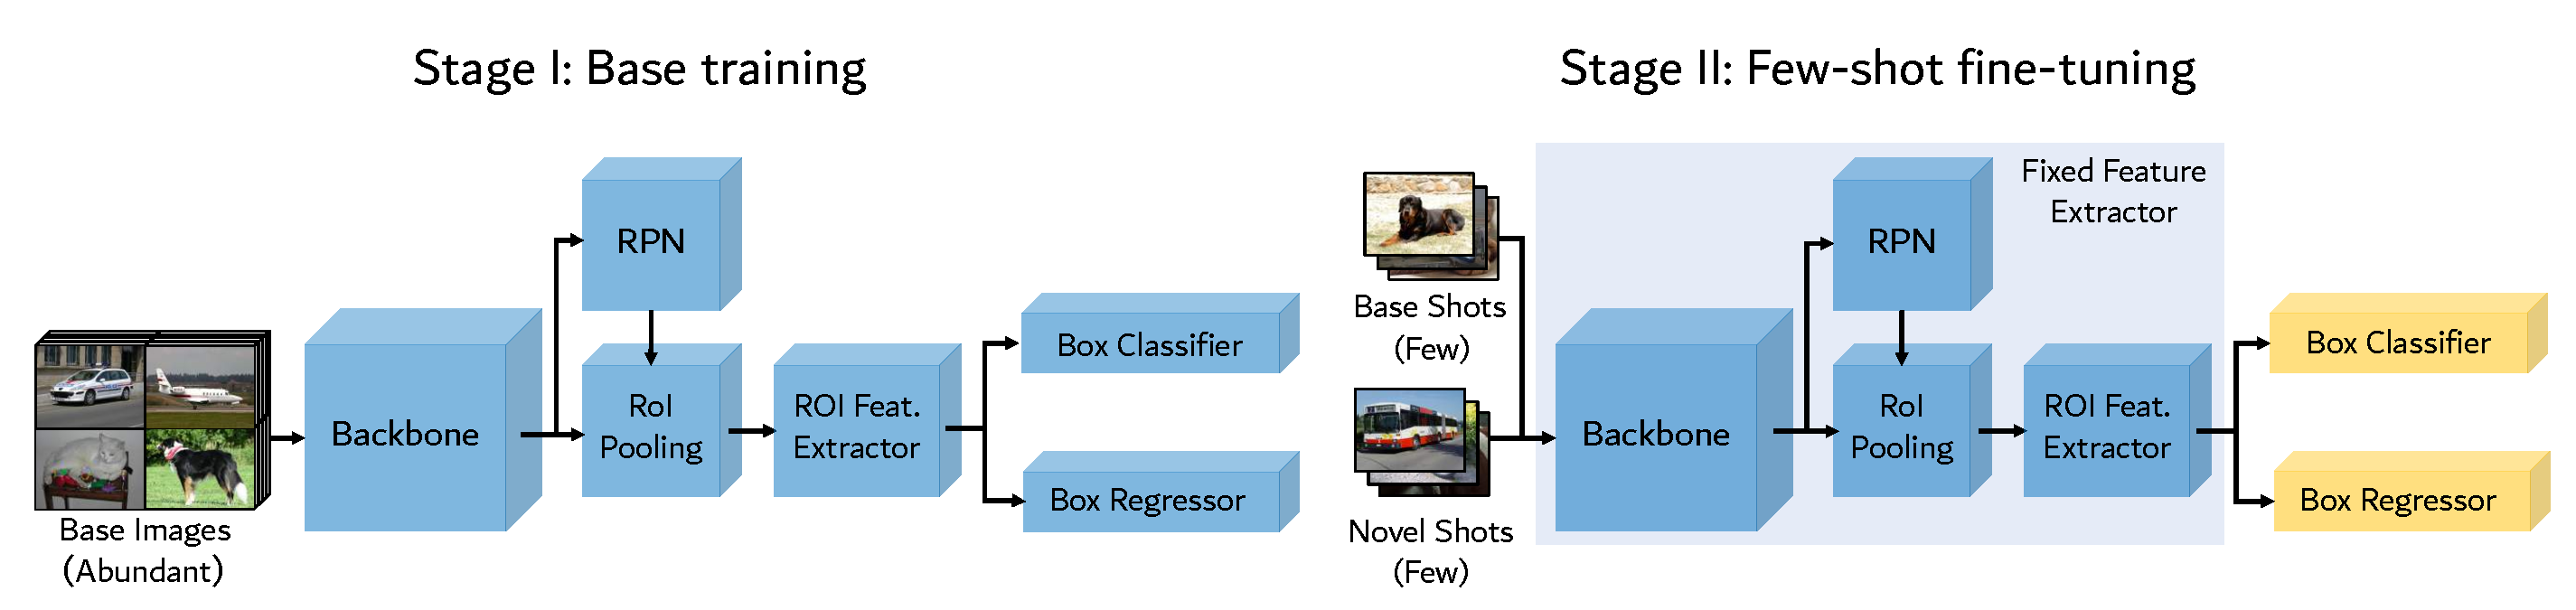
\includegraphics[width=\linewidth]{figs/TFA_fig1.pdf}
    \vspace{-1cm}
    \caption{Illustration of our two-stage fine-tuning approach (\model). In the base training stage, the entire object detector, including both the feature extractor $\mathcal{F}$ and the box predictor, are jointly trained on the base classes. In the few-shot fine-tuning stage, the feature extractor components are fixed and only the box predictor is fine-tuned on a balanced subset consisting of both the base and novel classes.}
    \label{fig:tfa_arch}
\end{figure*}

In this work, we propose improved methods to evaluate few-shot object detection. We carefully examine fine-tuning based approaches, which are 
considered to be under-performing in the previous works~\cite{kang2019few,yan2019meta,wang2019meta}.
% the standard baseline used in prior work 
We focus on the training schedule and the instance-level feature normalization of the object detectors in model design and training based on fine-tuning.

We adopt a two-stage training scheme for fine-tuning as shown in Figure~\ref{fig:tfa_arch}. We first train the entire object detector, such as Faster R-CNN~\cite{ren2015faster}, on the data-abundant base classes, and then only fine-tune the last layers of the detector
% (\textit{i.e.}, the fully connected layers used as the box classifier and the box regressor)
on a small balanced training set consisting of both base and novel classes while freezing the other parameters of the model. 
During the fine-tuning stage, we introduce instance-level feature normalization to the box classifier inspired by~\citet{gidaris2018dynamic,qi2018low,chen2019closer}. 


We find that this two-stage fine-tuning approach (\model) outperforms all previous
state-of-the-art meta-learning based methods by 2$\sim$20 points on the existing PASCAL
VOC~\cite{pascal-voc-2007} and COCO~\cite{Lin2014MicrosoftCC} benchmarks. 
When training on a single novel example (one-shot learning), our method can achieve twice
the accuracy of prior sophisticated state-of-the-art approaches.



Several issues with the existing evaluation protocols prevent consistent model comparisons. The accuracy measurements have high variance, making published comparisons unreliable.  Also, the previous evaluations only report the detection accuracy on the novel classes, and fail to evaluate knowledge retention on the base classes.
% encouraging knowledge forgetting on base classes.

To resolve these issues, we build new benchmarks on three datasets: PASCAL VOC, COCO and LVIS~\cite{gupta2019lvis}.
% disjoint groups
We sample different groups of few-shot training examples for multiple runs of the experiments to obtain a stable accuracy estimation and quantitatively analyze the variances of different evaluation metrics. The new evaluation reports the average precision (AP) on both the base classes and novel classes as well as the mean AP on all classes, referred to as the generalized few-shot learning setting in the few-shot classification literature~\cite{hariharan2017low,wang2019tafe}.

Our fine-tuning approach establishes new states of the art on the benchmarks.  
On the challenging LVIS dataset, our two-stage training scheme improves the average detection precision of rare classes
($<$10 images) by $\sim$4 points and common classes (10-100 images) by $\sim$2 points with negligible precision loss for the frequent classes ($>$100 images). 
